\documentclass[12pt]{ctexart}
\usepackage{graphicx}%图片引用包
\usepackage{amssymb}%特殊符号
\usepackage{amsmath}%矩阵
\usepackage{amsthm}%定理
\usepackage{geometry}%缩放
\usepackage{hyperref}%超链接
\usepackage{framed}%框框
\usepackage{mathrsfs}%花体
\usepackage{anyfontsize}
\usepackage{indentfirst}%缩进
\usepackage{extsizes}%size
\usepackage{newtxtext,newtxmath}%times风格字体



\setlength{\parindent}{2em}%缩进参数
\linespread{1.55}%行间距
\geometry{a4paper,scale=0.75}%大小



\newtheorem{thm}{Theorem}[section]

\hypersetup
    {
        colorlinks=true,
        linkcolor=blue,
        anchorcolor=blue,
        citecolor=blue
    }%超链接

\title{Fluorescence Lifetime Imaging Technique Notes\\荧光寿命成像技术笔记}
\author{Jerry Ling} 
\date{\today}
 


\begin{document}  %begin后括号内是文件类型
\maketitle  %生成标题
The technique we are introducing based on the process of molecular \textbf{fluorescence}, an emitting process after excitement. Generally, a simple fluorescence process is an 1-order exponentially decaying funtion w.r.t. time, whose decaying constant tells a lot of story about its surroundings or status. This infomation could be used to image or to explore dynamics of molecular. To begin with, we shall first introduce the techniques of measuring, then the theory about fluorescence process and quenching, finally the selected applications. 
\begin{framed}
    This note emphasizes the framework and main line, with some additional deriving, so combined reading with the original paper is suggested. 
\end{framed}
\section{Measurement of Fluorescence Lifetime}
\subsection*{Early development}
\par The very first problem for Fluorescence Lifetime imaging is the Measurement of super-short time interval, say between 2 pulses of light. At the beginning people could only measure the lifetime of \textbf{phosphorescent(磷光)} whose scale on minute or hour by raw eye, until recently new methods was developed:
\begin{itemize}
    \item [$\bullet$] E. Becquerel (1859) introduced rotating wheel to measure light decay down to $10^{-4}s$. The point is to use \textbf{linear velocity} $v=R\omega$ to replace normal ones. 
    \item [$\bullet$] John Kerr (1875) discovered \textbf{Kerr effect} and Abraham \& Lemoine (1899) use the \textbf{Kerr’s cell} to measure ultrafast time interval. \textbf{Synchronization(共时激发)} triggers off both the depolarization (2.7ns) of Kerr cell and the light to be measured. The later is \textbf{modulated} by a filter, and its phase-shift (caused by \textbf{polarized} Kerr cell) is measured to count time. 
    \item [$\bullet$] Finally, E. Gaviola (1926) combined the two apparatus and established the prototype of modern devices for fluorescence lifetime measurement, normally refered to as \textbf{fluorometer}.
\end{itemize}
\subsection*{Data Acquisition}
\par Besides time-measurement, modern devices follow diffenent technical path to obtain lifetime information. 
Time domain detection relies on \textbf{Time-correlated single photon counting(TCSPC)}, where a pluse (1-2 ns) triggers off a stream of photons, who then reaches a photomultiplier tube and go through a \textbf{Time-to-Digital Converter} to be stamped with time. Counting the numbers w.r.t time and repeat the pulse to take average gives the time domain spectrum. A fitting then gives the constant we want:
\begin{framed}
    \begin{equation}
        I=I_0e^{-\frac{t}{\tau}}
        \label{decay_equ}
    \end{equation}
\end{framed}
\begin{framed}
    \noindent Note that the number of photons could be corrected by calculating variance of wait time, since this process could be modeled as a \textbf{poisson process}.
\end{framed}

\par Frequency domain spectrum is theoritically identical with time domain specturm by FT. The incident light is modulated at high frequency $\omega_0$, then convolute with form of (\ref{decay_equ}). The output is also going to oscillate at $\omega_0$ but experience a \textbf{phase shift(相移)}$\varphi$ and a \textbf{demodulation(去调制)}$M$ as a function of lifetime. To see this, we first calculate the fourier transform of input signal and \textbf{response function(系统响应函数)} [the output given x(t)=$\delta(t)$]:
\begin{equation}
    \mathscr{F}[I_0e^{-\frac{t}{\tau}}]=H(j\omega)=I_0\frac{1}{\frac{1}{\tau}+j\omega},t>0
    \label{response_func}
\end{equation}
\begin{equation}
    \mathscr{F}[sin(\omega_0t)]=X(j\omega)=j\pi[\delta(\omega+\omega_0)-\delta(\omega-\omega_0)]
\end{equation}
Multiple them to get the output domain spectrum(convolution theorem):
\begin{equation}
    Y(i\omega)=j\pi I_0\frac{\delta(\omega\pm\omega_0)}{1/\tau+j\omega_0}
\end{equation}
The delta fuction ensures that output oscillate at frequency $\omega_0$, while taking the angle part of (\ref{response_func}) gets the phase shift:
\begin{equation}
    H(j\omega)=I_0\frac{1/\tau-j\omega}{{1}/\tau^2+\omega^2}
\end{equation}
\begin{framed}
    \begin{equation}
        tan(\varphi)=-\omega\tau
    \end{equation}
\end{framed}
\noindent $H(j\omega)$ is called \textbf{Frequency Response Function(频率响应函数)}, whose the module and angle shows the change by the corresponding system on input. Demodulation may be derived in a similar way.
\subsection*{Anisotropy}
(wait to be done)
\subsection*{Multi-photon excitation}
\begin{itemize}
    \item excited to 2$\lambda$ state
    \item requires high flux (100 $MW/cm^2$ to 100 $ GW/cm^2$) produced by pm/fm lasers
    \item short pulse: no photodestruction of the molecules
    \item increased spatial resolution——mainstay of fluorescence lifetime imaging microscopy (FLIM)
\end{itemize}
\subsection*{*Second harmonic generation (SHG)}
\begin{itemize}
    \item incident light at $\lambda$ is 'converted' to 2$\lambda$
    \item does \textbf{not} proceed through an excited state; no energy is lost through nonradiative pathways
    \item Schenke-Layland, K. J. Biophotonics 2008, 1, 451.
\end{itemize}
\begin{framed}
    Note: this technique relies on \textbf{nonlinear optics(非线性光学)} and does not depend on fluorescence lifetime thus won't be discussed here.
\end{framed}

\section{Theory of Fluorescence Lifetime and Processes}
\par Now we shall develop the general theory about fluorescence lifetime. We will go through the following 3 questions: Energy pathways(kinetics)? Spontaneous decay? Quenching ways?
\subsection*{Energy pathways}
The fate of absorbed energy could be showed in one famous diagram, see Fig \ref{Jablonski_diagram}.
\begin{figure}[t]
    \centering
    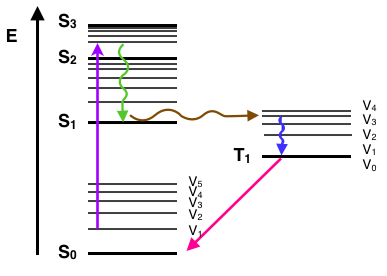
\includegraphics[width=0.4\textwidth]{Jablonski diagram.png}
    \caption{Jablonski diagram}
    \label{Jablonski_diagram}
\end{figure}
The process from S1 to S0 emits fluorescence, but the decay of which depends on all processes leaving S1. Since most of them obey first-order decaying equation, lifetime could be written as:
\begin{equation}
    \tau=\frac{1}{k_f+k_{nr}}
\end{equation}
\noindent Those other then fluorescence is called nonradiative process. Clearly the less of them, the longer is lifetime. 
\par To measure the ability/probability to emit fluorescence, define \textbf{Quantum Yield} by the part of absorbed light turns into fluorescence: $\Phi=\frac{n_{f}}{n_{abs}}$. This is equal to ratio of decay constants of nature emission and measured emission. The former could be calculated by absorption and emission spectrum, as will be explained later.

\subsection*{Nature emission}
It turns out that the \textbf{nature emission}(without any quenching process) has dependence on wavelength. In the case where absorption and emission shares one wavelength, Einstein derived the expression of Spontaneous emission by setting equilibrium:
\begin{equation}
    A_{10}=\frac{1}{\tau_{nature}}=\frac{8\pi h}{\lambda^3}B_{01}
\end{equation}
Where $B_{01}=B_{10}$ is the \textbf{induced transition probability(受激跃迁几率)}. The highlight of this theory is to take in consideration of induced emission, which shares phase, direction and frequency with incident light. Though useful in laesr producing, this cannot be directly applied to fluorescence research since the later emits light different from absorbed. 
\par The version for fluorescence is established by Strickler and Berg(1962). Under rigid rotor assumption, they relate $\tau_n$ with experimentally accessible data as reflection index and absorption:
\begin{equation}
    1 / \tau_{\mathrm{n}}=2.880 \times 10^{-9} n^{2}\left\langle\widetilde{\nu}_{f}^{-3}\right\rangle_{Av}^{-1}\left(g_{1} / g_{u}\right) \int \epsilon(v) \mathrm{d} I n \widetilde{\nu}
\end{equation}
This theoritical lifetime may serve as an indicator for the sensitivity of molecular to the environment. To dig deeper into the factors, we will explore the process of quenching:
\subsection*{Internal quenching}
Internal quenching stems from local change around fluorescence group. 3 main sources will lead to internal quenching, some of them are sensitive to the environment, thus have the potential to serve as the corresponding probes.
\begin{figure}[t]
    \centering
    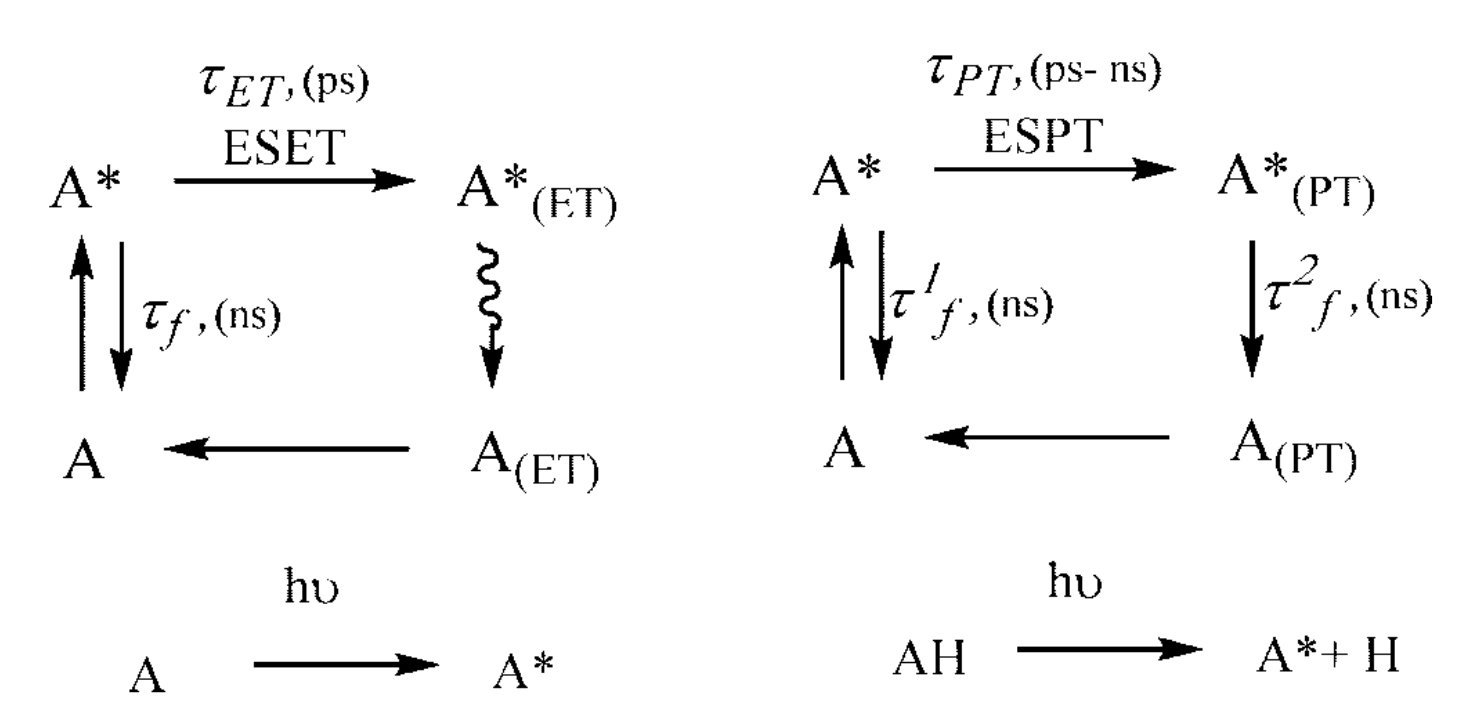
\includegraphics[width=0.7\textwidth]{ESET_ESPT.png}
    \caption{ESET and ESPT}
    \label{ESET_ESPT}
\end{figure}
\begin{itemize}
    \item Intramolecular rotation (IMR, 分子内扭转): \underbar{viscosity, temperature,polarity and electron} \\ \underbar{structure} may affect rotation. For barrierless rotor: $k_{rot}=\frac{1}{\theta_r}=\frac{k_B T}{4\pi r^3\eta}$ .
    \item Excited state electron/proton transfer (ESET/ESPT): Due to \textbf{revisible} electron distribution change, less sensitive to environment. See Fig \ref{ESET_ESPT}.
    \item Intersystem crossing: Due to spin-orbital coupling (S$\to$T). Heavy atoms have more intersystem crossing.
    
\end{itemize}
\subsection*{External quenching}
External quenching, in the contrast, is due to the environment or other part of the macromolecular. Among them, FRET plays a significant role in researches. We shall also develop some formulas to better utilize these phenomenons.
\begin{itemize}
    \item Forster Resonance Energy Transfer (FRET): Due to \textbf{dipole interaction}, whose efficiency is a function of distance $r$ between accepter and donor: $E_t=\frac{R_0^6}{R_0^6+r^6}*100\%$. $R_0$ could be calculated with spectrum information. See Fig \ref{FRET}.
    \item Dexter Electron Transfer (DET): Due to electron overlap. Increase exponentially w.r.t distance.
    \item Dynamic quenching: Due to collision. The nonradiative molecules are called \textbf{Quenchers}. \textbf{Stern-Volmer equation} describes the effect on lifetime: $\tau=\tau_0/(1+k_Q\tau_0[Q])$. The constant could be derived considering diffusion process: $k_{\mathrm{q}}=\frac{8 r_{\mathrm{AQ}} T}{3 \eta} \times \frac{N_{\mathrm{A}}}{1000} \times p$. Certain small molecules like \underbar{iodine and oxygen} have a high probability of quenching (p$\to$1).
    \item Reabsorption: Occurs when concentration is too high. Lifetime increases and then decreases due to reactions of nonradiative products.
    \item Excimer: Excited molecule associates with \textbf{the same} molecule in the ground state. Appears an extra emission spectrum distinct from the monomer.
\end{itemize}
\begin{figure}[t]
    \centering
    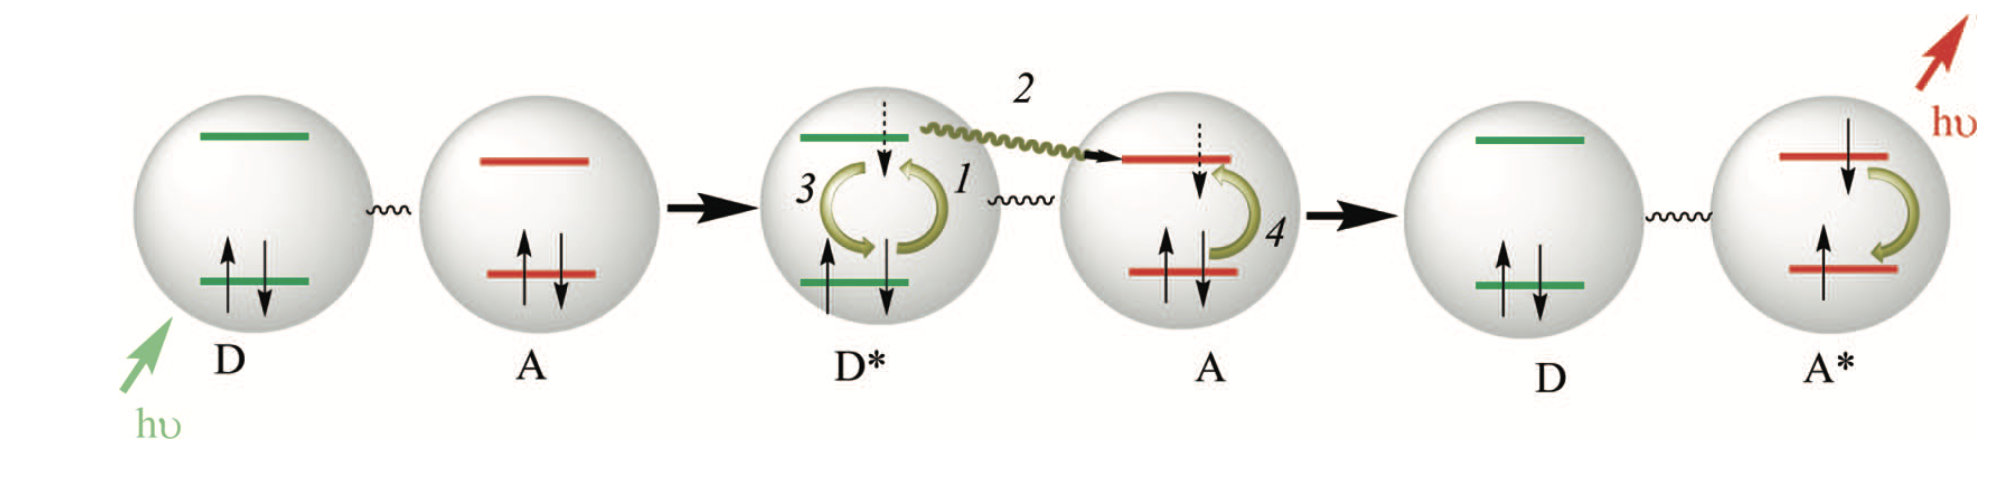
\includegraphics[width=0.7\textwidth]{FRET.png}
    \caption{FRET process}
    \label{FRET}
\end{figure}

\section{Common Molecules and Applications}
This section involves a wide range of probes and moleculars. The principle is to first know what you need, then go for the candidates that have the suitable property, such as the sensitivity to pH, oxygen or polarity. See Fig \ref{probes}. To appreciate the applications one may refer to the origin literature and the cites, for there are too much to be reviewed.
\begin{figure}[t]
    \centering
    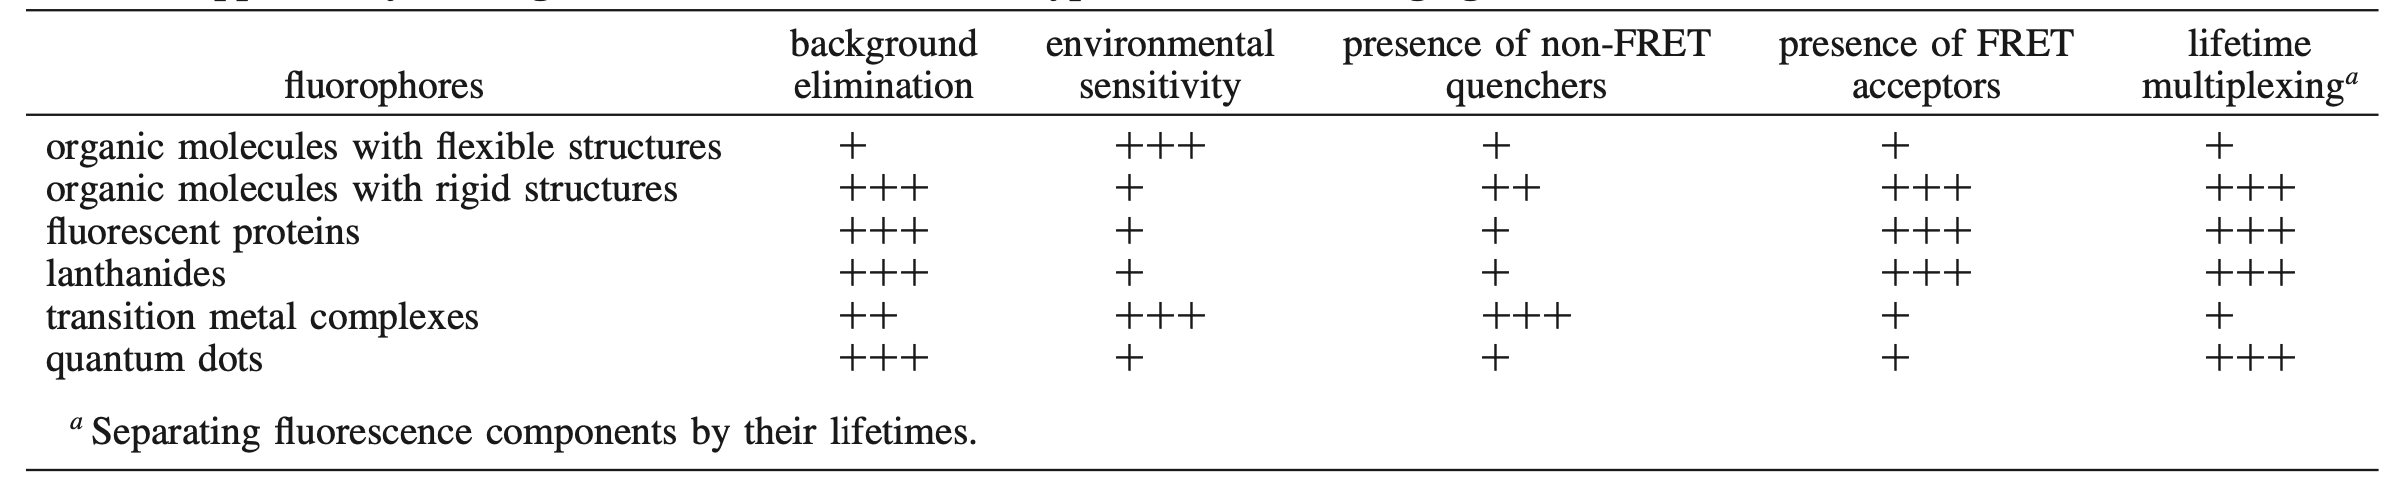
\includegraphics[width=1.0\textwidth]{Probes.png}
    \caption{Comparison between probes}
    \label{probes}
\end{figure}
\subsection*{Autofluorescence}
Note that Autofluorescence sometimes cause background noise.
\begin{itemize}
    \item Amino Acids: tryptophan is mostly used, sensitive to environment.
    \item NADH: free rotation between the pyridine and amide, sensitive to environment
    \item Flavin adenine dinucleotide: only the non-bound form of FAD is fluorescent
    \item Porphyrins(卟啉类)
    \item Melanin(黑色素)
    \item Lipofuscin(脂褐素)
    \item Collagen and Elastin
\end{itemize}
\subsection*{Exogenous Fluorescence Molecular}
\begin{itemize}
    \item Small Organic Fluorophores
    \item Fluorophore proteins
    \item Quantum dots
    \item Metal-Based probes: MLCT; Complexes of Lanthanides; UpConversion
\end{itemize}


\end{document}